% =============================================================================
% 04_results.tex - Results
% =============================================================================

\section{Results}
\label{sec:results}

\subsection{Overview of Clustering Performance}

We evaluated Seurat/Leiden clustering at five resolution parameters, SC3 consensus clustering (scMixology only), and recall FDR-controlled clustering across three benchmark datasets. Table~\ref{tab:metrics_summary} presents the primary clustering metrics for representative methods.

\begin{table}[htbp]
\centering
\caption{Summary of clustering performance across datasets. $K$: number of clusters identified; ARI: Adjusted Rand Index; NMI: Normalized Mutual Information; OCI: Overclustering Index. Best ARI for each dataset shown in bold. SC3 results available only for scMixology due to memory constraints.}
\label{tab:metrics_summary}
\begin{tabular}{@{}llccccc@{}}
\toprule
\textbf{Dataset} & \textbf{Method} & \textbf{K} & \textbf{K$_{\text{true}}$} & \textbf{ARI} & \textbf{NMI} & \textbf{OCI} \\
\midrule
\multirow{4}{*}{scMixology}
    & Leiden (res=0.2) & 4 & 3 & \textbf{0.856} & 0.812 & 0.33 \\
    & Leiden (res=0.8) & 7 & 3 & 0.545 & 0.576 & 1.33 \\
    & SC3 & 5 & 3 & 0.741 & 0.699 & 0.67 \\
    & recall & 6 & 3 & 0.680 & 0.649 & 1.00 \\
\midrule
\multirow{3}{*}{PBMC 3k}
    & Leiden (res=0.8) & 8 & 9 & 0.780 & 0.836 & $-$0.11 \\
    & Leiden (res=1.0) & 8 & 9 & \textbf{0.781} & 0.837 & $-$0.11 \\
    & recall & 7 & 9 & 0.649 & 0.728 & $-$0.22 \\
\midrule
\multirow{3}{*}{Zeisel}
    & Leiden (res=0.2) & 4 & 7 & \textbf{0.797} & 0.692 & $-$0.43 \\
    & Leiden (res=0.8) & 7 & 7 & 0.425 & 0.590 & 0.00 \\
    & recall & 8 & 7 & 0.481 & 0.597 & 0.14 \\
\bottomrule
\end{tabular}
\end{table}

\subsection{scMixology Dataset: Simple Ground Truth}

The scMixology dataset, consisting of three well-separated cell lines, provides an ideal test case for evaluating clustering accuracy. Leiden clustering at low resolution (0.2) achieved the highest accuracy (ARI = 0.856), despite identifying four clusters rather than the true three. SC3 consensus clustering achieved ARI = 0.741 with five predicted clusters, while recall obtained ARI = 0.680 with six clusters.

The superior performance of low-resolution Leiden on this dataset reflects the well-separated nature of the cell populations. Higher resolution values (0.8, 1.0, 1.5) led to substantial overclustering, fragmenting the biologically coherent populations into multiple spurious clusters (Figure~\ref{fig:ari_comparison}).

\begin{figure}[htbp]
\centering
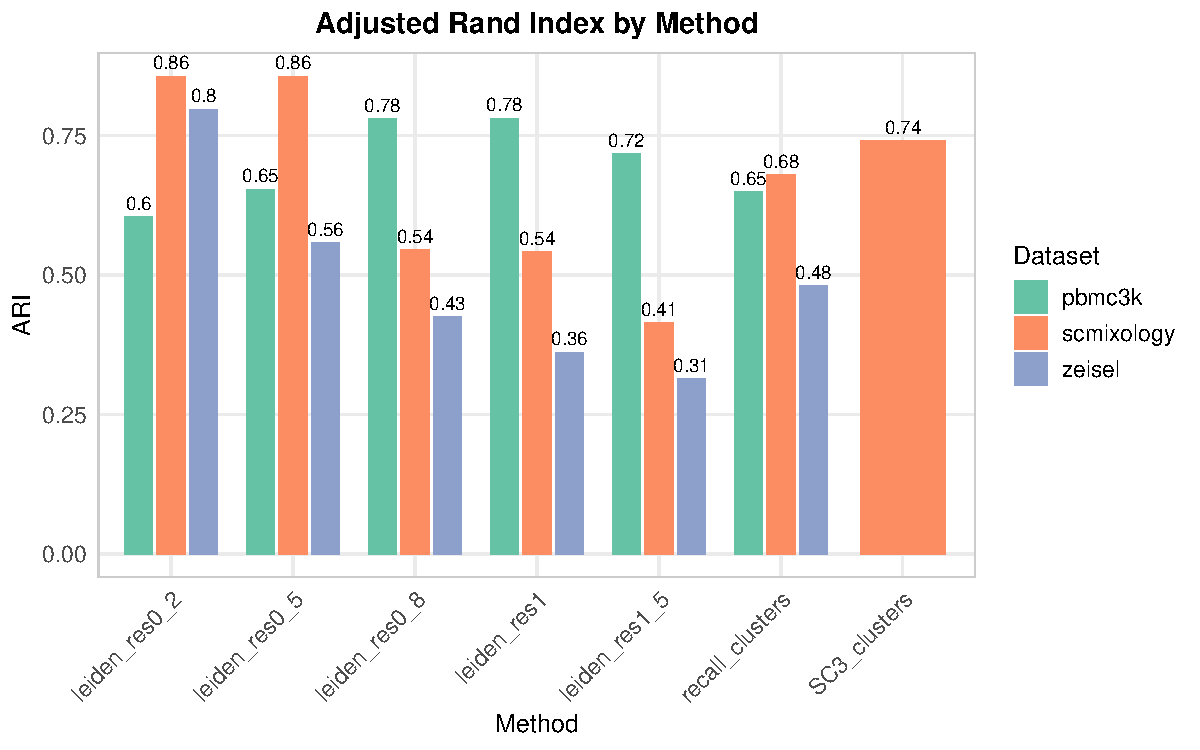
\includegraphics[width=0.9\textwidth]{figures/ari_comparison.pdf}
\caption{Adjusted Rand Index (ARI) comparison across methods and datasets. Higher values indicate better agreement with ground truth labels. Leiden results shown for multiple resolution values (0.2, 0.5, 0.8, 1.0, 1.5). SC3 results available only for scMixology. The optimal resolution varies by dataset: scMixology and Zeisel favor low resolution, while PBMC 3k favors moderate resolution.}
\label{fig:ari_comparison}
\end{figure}

\subsection{PBMC 3k Dataset: Immune Cell Complexity}

The PBMC 3k dataset presents greater complexity with nine distinct immune cell types. Here, moderate resolution Leiden clustering (0.8--1.0) achieved the best performance (ARI = 0.781), correctly identifying eight of nine cell types. The slightly negative OCI ($-$0.11) indicates minor underclustering, with one cell type likely merged with a similar population.

recall achieved ARI = 0.649 with seven predicted clusters, reflecting its conservative merging behavior. The FDR control mechanism merged clusters that did not meet the significance threshold, resulting in underclustering relative to the ground truth (Figure~\ref{fig:nmi_comparison}).

\begin{figure}[htbp]
\centering
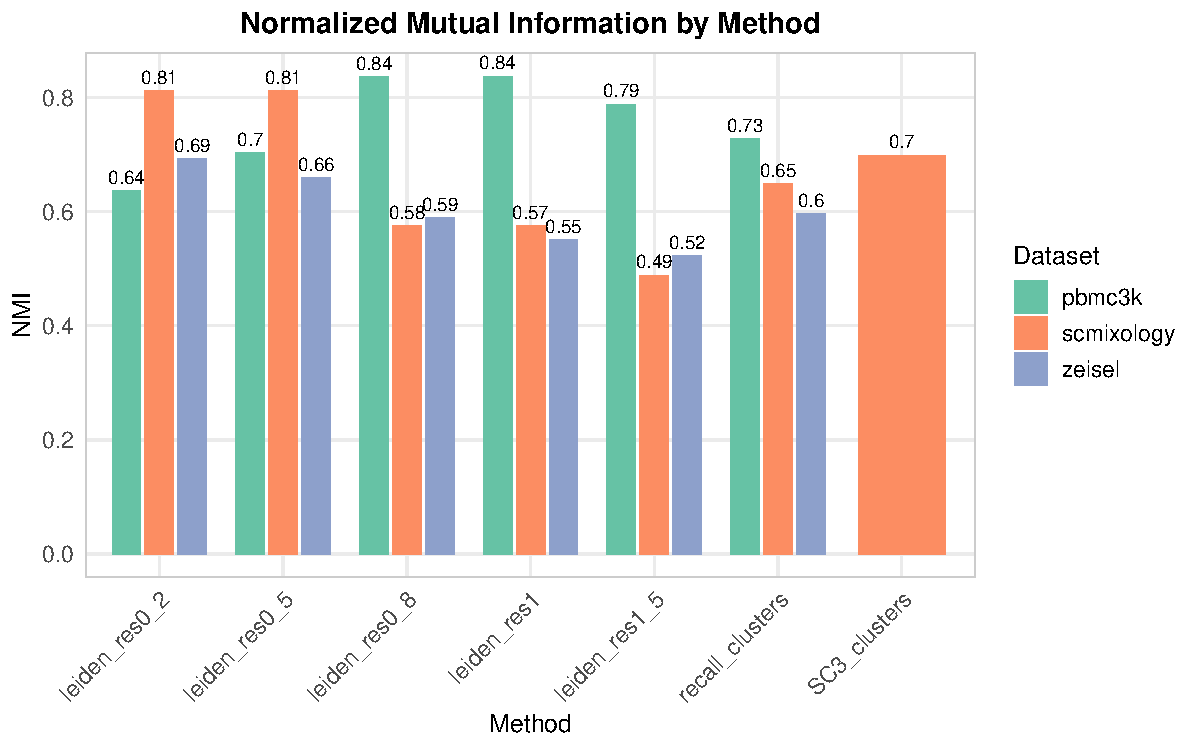
\includegraphics[width=0.9\textwidth]{figures/nmi_comparison.pdf}
\caption{Normalized Mutual Information (NMI) comparison across methods and datasets. NMI values correlate strongly with ARI but provide an information-theoretic perspective on clustering quality. Higher values indicate greater shared information between predicted and true cluster labels.}
\label{fig:nmi_comparison}
\end{figure}

\subsection{Zeisel Brain Dataset: Hierarchical Structure}

The Zeisel dataset, with its hierarchical structure of neuronal and glial cell types, revealed an interesting pattern. Low-resolution Leiden (0.2) achieved the highest ARI (0.797) despite identifying only four clusters versus the true seven. This counterintuitive result suggests that the level1 annotation may not represent the optimal clustering granularity for this dataset---the four predicted clusters may correspond to biologically meaningful groupings at a coarser level.

Higher resolution values that matched the ground truth cluster count ($K=7$ at resolution 0.8) achieved lower ARI (0.425), indicating that forcing the correct number of clusters does not guarantee correct cluster assignments. recall achieved ARI = 0.481 with eight predicted clusters.

\subsection{Cluster Count Analysis}

Figure~\ref{fig:cluster_counts} illustrates the relationship between resolution parameter and predicted cluster count across datasets. As expected, cluster count increases monotonically with resolution for Leiden clustering. The ground truth cluster count is indicated for reference.

\begin{figure}[htbp]
\centering
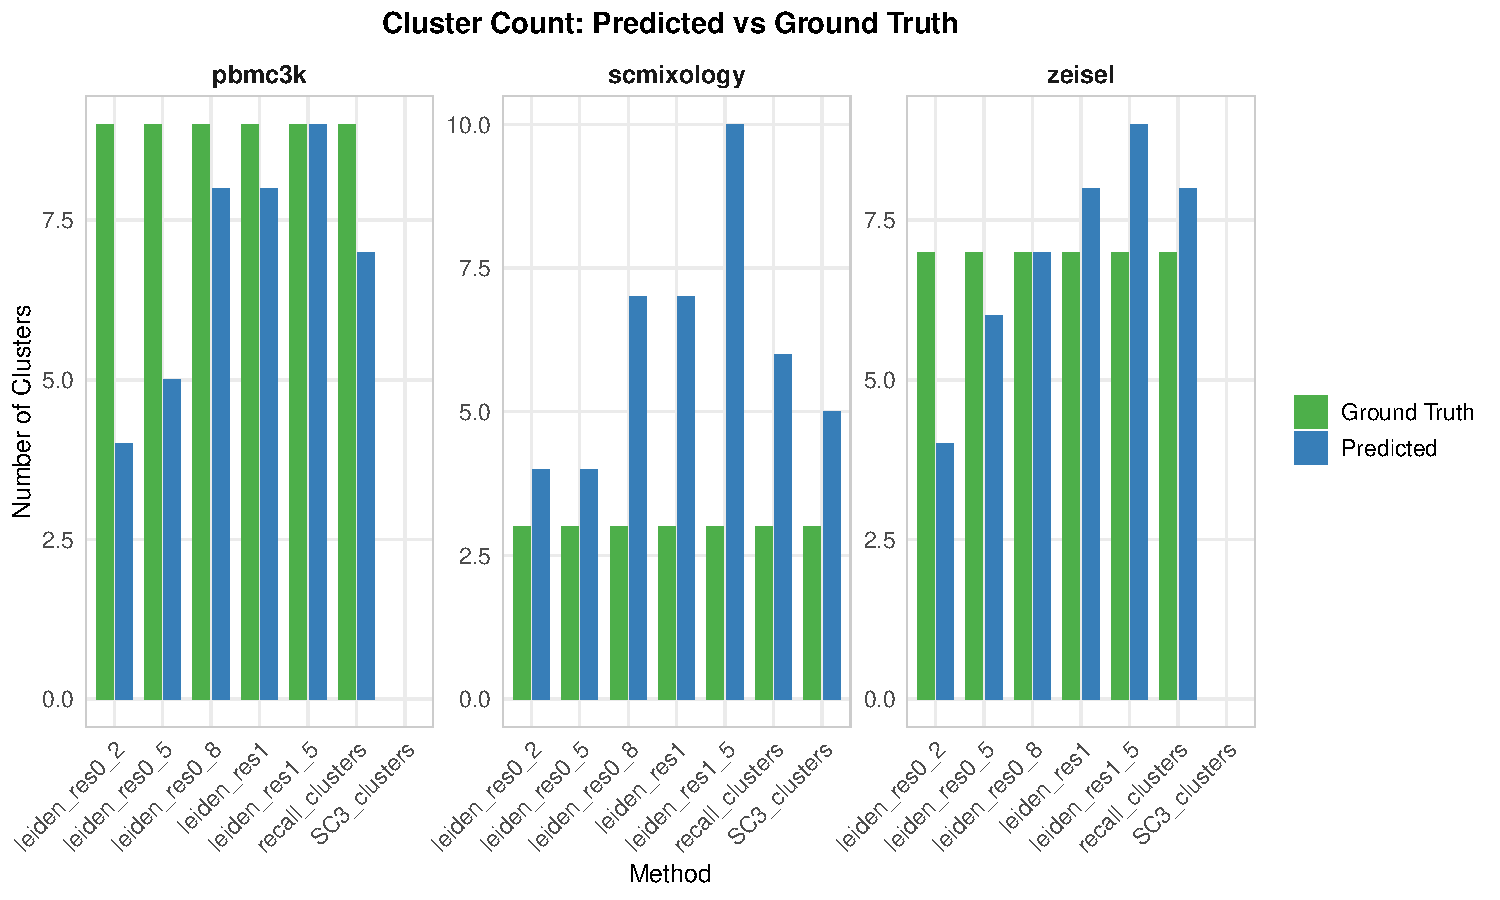
\includegraphics[width=0.85\textwidth]{figures/cluster_counts.pdf}
\caption{Number of clusters identified by each method across datasets. Horizontal dashed lines indicate ground truth cluster counts (scMixology: 3, PBMC 3k: 9, Zeisel: 7). Leiden cluster counts increase with resolution. SC3 and recall provide single predictions per dataset without resolution tuning.}
\label{fig:cluster_counts}
\end{figure}

\subsection{Overclustering Analysis}

The overclustering index (OCI) quantifies the tendency of methods to over- or under-partition the data (Figure~\ref{fig:overclustering}). For scMixology, all methods exhibited positive OCI, with Leiden at resolution 1.5 showing the most severe overclustering (OCI = 2.33, corresponding to 10 clusters vs. 3 true). For PBMC 3k, moderate underclustering was observed across methods. For Zeisel, low-resolution Leiden substantially underclustered (OCI = $-$0.43), while higher resolutions approached the ground truth count.

\begin{figure}[htbp]
\centering
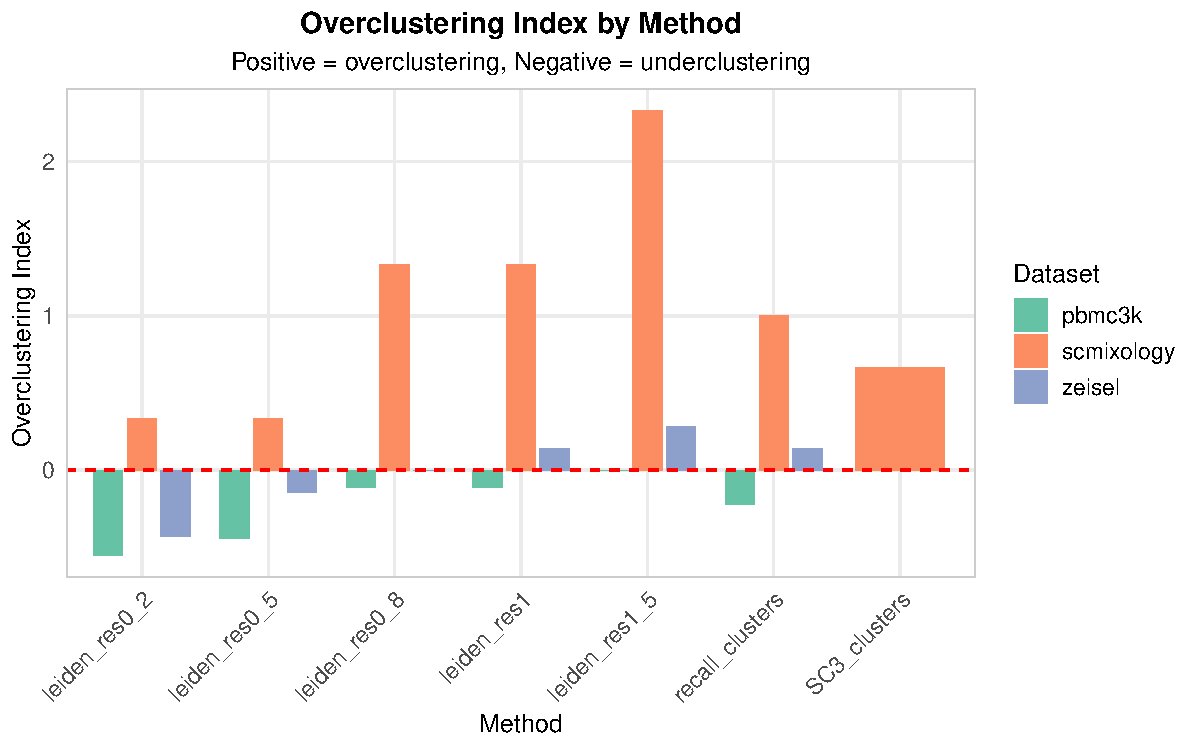
\includegraphics[width=0.85\textwidth]{figures/overclustering_analysis.pdf}
\caption{Overclustering Index (OCI) by method and dataset. OCI = $(K_{\text{predicted}} - K_{\text{true}}) / K_{\text{true}}$. Positive values indicate overclustering; negative values indicate underclustering; zero indicates exact cluster count match. Statistical calibration methods (SC3, recall) show varying behavior depending on dataset complexity.}
\label{fig:overclustering}
\end{figure}

\subsection{UMAP Visualization}

UMAP~\cite{mcinnes2018umap} visualizations provide qualitative assessment of clustering quality. Figure~\ref{fig:umap_scmixology} shows the scMixology results, where the three cell lines form clearly separated clusters. Leiden at low resolution correctly identifies these populations, while higher resolutions fragment them into multiple clusters.

\begin{figure}[htbp]
\centering
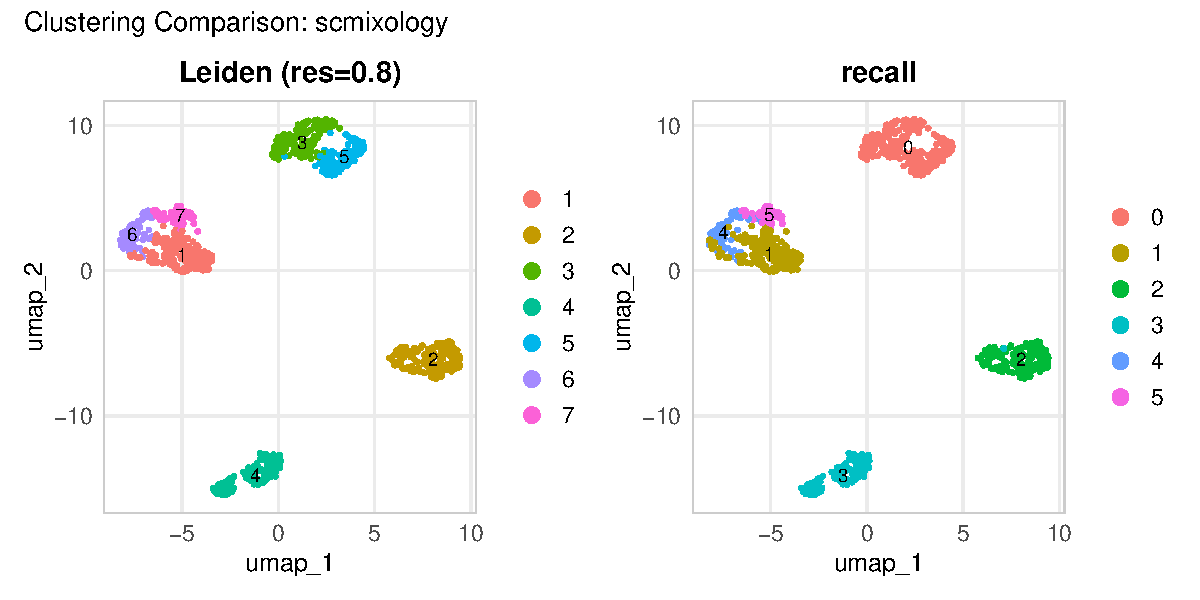
\includegraphics[width=0.9\textwidth]{figures/umap_scmixology.pdf}
\caption{UMAP visualization of scMixology clustering results. The three cell lines (HCC827, H1975, H2228) form well-separated clusters in the embedding space. Panel A shows ground truth labels; subsequent panels show predicted clusters from different methods. Color coding indicates cluster assignment.}
\label{fig:umap_scmixology}
\end{figure}

The PBMC 3k and Zeisel datasets show more complex structure with overlapping populations (Figures~\ref{fig:umap_pbmc3k} and~\ref{fig:umap_zeisel}), explaining the greater challenge in achieving high clustering accuracy.

\begin{figure}[htbp]
\centering
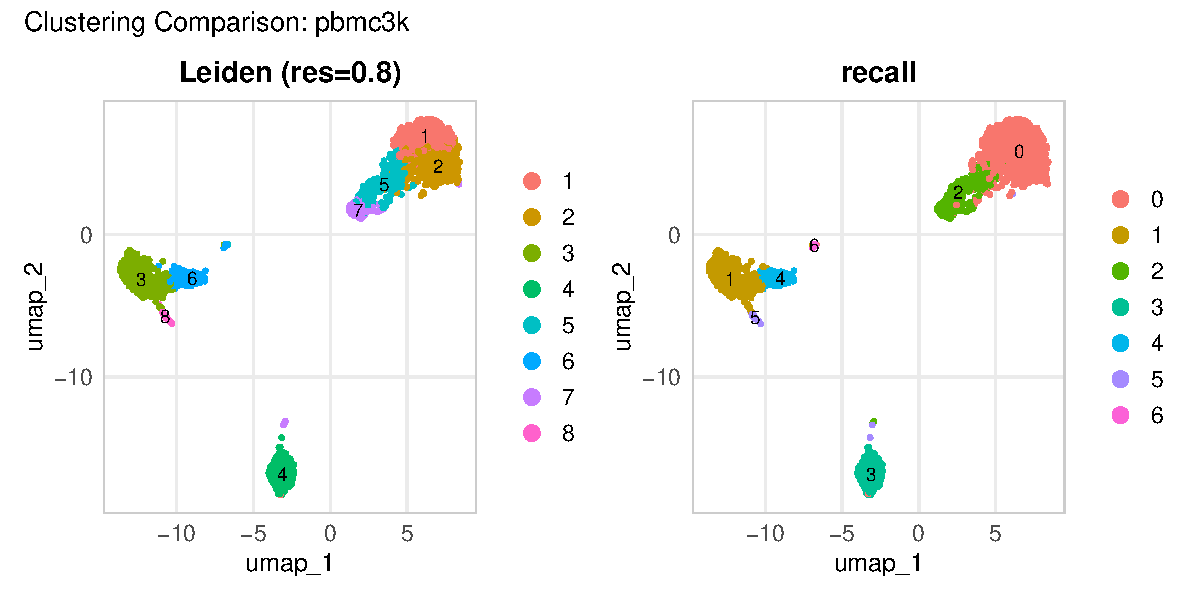
\includegraphics[width=0.9\textwidth]{figures/umap_pbmc3k.pdf}
\caption{UMAP visualization of PBMC 3k clustering results. Nine immune cell types show varying degrees of separation, with some populations (e.g., CD4+ and CD8+ T-cells) exhibiting overlapping expression profiles. Monocyte and NK cell populations are well separated.}
\label{fig:umap_pbmc3k}
\end{figure}

\begin{figure}[htbp]
\centering
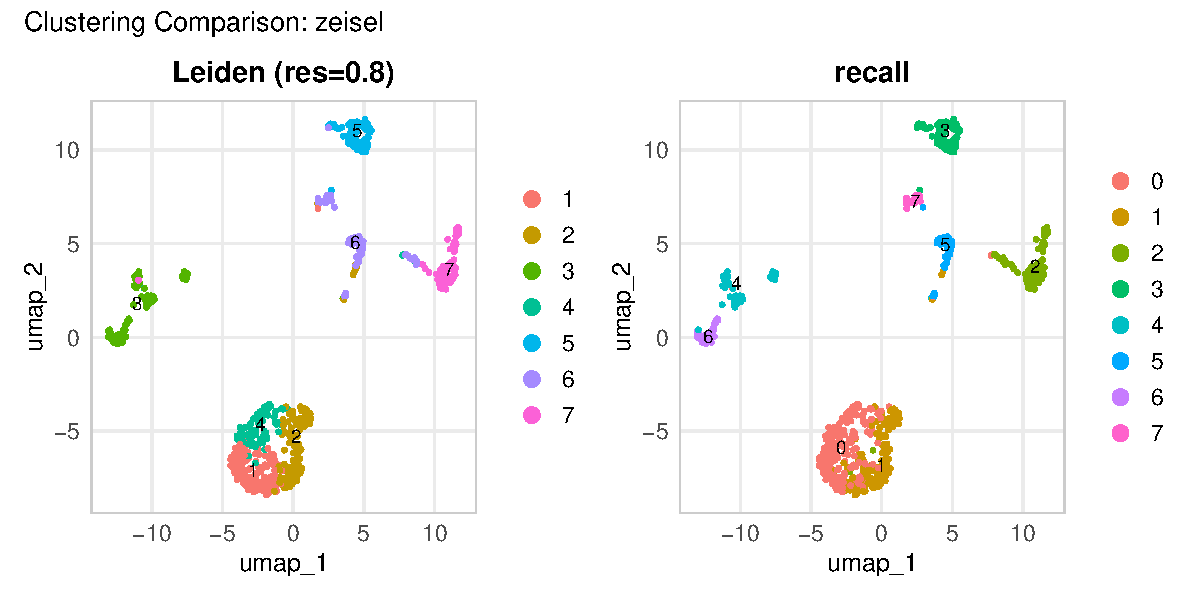
\includegraphics[width=0.9\textwidth]{figures/umap_zeisel.pdf}
\caption{UMAP visualization of Zeisel brain dataset clustering results. Seven major cell classes at the level1 annotation show hierarchical structure, with neuronal and glial populations occupying distinct regions of the embedding space.}
\label{fig:umap_zeisel}
\end{figure}

\subsection{Extended Metrics}

Table~\ref{tab:extended_metrics} presents the complete set of clustering metrics for all methods and datasets.

\begin{table}[htbp]
\centering
\caption{Extended clustering metrics for all methods. Homog.: Homogeneity; Compl.: Completeness; Silh.: Silhouette Score.}
\label{tab:extended_metrics}
\small
\begin{tabular}{@{}llcccccc@{}}
\toprule
\textbf{Dataset} & \textbf{Method} & \textbf{K} & \textbf{ARI} & \textbf{NMI} & \textbf{Homog.} & \textbf{Compl.} & \textbf{Silh.} \\
\midrule
\multirow{7}{*}{scMixology}
    & Leiden 0.2 & 4 & 0.856 & 0.812 & 0.987 & 0.812 & 0.354 \\
    & Leiden 0.5 & 4 & 0.856 & 0.812 & 0.987 & 0.812 & 0.354 \\
    & Leiden 0.8 & 7 & 0.545 & 0.576 & 0.988 & 0.576 & 0.212 \\
    & Leiden 1.0 & 7 & 0.542 & 0.575 & 0.988 & 0.575 & 0.211 \\
    & Leiden 1.5 & 10 & 0.415 & 0.489 & 0.989 & 0.489 & 0.178 \\
    & SC3 & 5 & 0.741 & 0.699 & 0.982 & 0.699 & 0.268 \\
    & recall & 6 & 0.680 & 0.649 & 0.982 & 0.649 & 0.290 \\
\midrule
\multirow{6}{*}{PBMC 3k}
    & Leiden 0.2 & 4 & 0.604 & 0.637 & 0.637 & 0.948 & 0.232 \\
    & Leiden 0.5 & 5 & 0.654 & 0.703 & 0.703 & 0.935 & 0.231 \\
    & Leiden 0.8 & 8 & 0.780 & 0.836 & 0.836 & 0.838 & 0.128 \\
    & Leiden 1.0 & 8 & 0.781 & 0.837 & 0.837 & 0.838 & 0.128 \\
    & Leiden 1.5 & 9 & 0.717 & 0.788 & 0.843 & 0.788 & 0.102 \\
    & recall & 7 & 0.649 & 0.728 & 0.728 & 0.935 & 0.236 \\
\midrule
\multirow{6}{*}{Zeisel}
    & Leiden 0.2 & 4 & 0.797 & 0.692 & 0.692 & 0.819 & 0.315 \\
    & Leiden 0.5 & 6 & 0.558 & 0.660 & 0.781 & 0.660 & 0.183 \\
    & Leiden 0.8 & 7 & 0.425 & 0.590 & 0.785 & 0.590 & 0.128 \\
    & Leiden 1.0 & 8 & 0.362 & 0.551 & 0.787 & 0.551 & 0.110 \\
    & Leiden 1.5 & 9 & 0.315 & 0.523 & 0.791 & 0.524 & 0.095 \\
    & recall & 8 & 0.481 & 0.597 & 0.790 & 0.597 & 0.140 \\
\bottomrule
\end{tabular}
\end{table}

Notable observations from the extended metrics:
\begin{itemize}[noitemsep]
    \item \textbf{Homogeneity} remains high ($>0.98$) for scMixology across all methods, indicating that predicted clusters consistently contain cells from the same true population
    \item \textbf{Completeness} decreases with increasing resolution, as overclustering splits true populations across multiple predicted clusters
    \item \textbf{Silhouette scores} decrease with higher resolution, reflecting less well-defined cluster boundaries when data is over-partitioned
\end{itemize}
